\documentclass{standalone}
\usepackage{tikz}
\usetikzlibrary{decorations.pathmorphing, arrows.meta}

\begin{document}

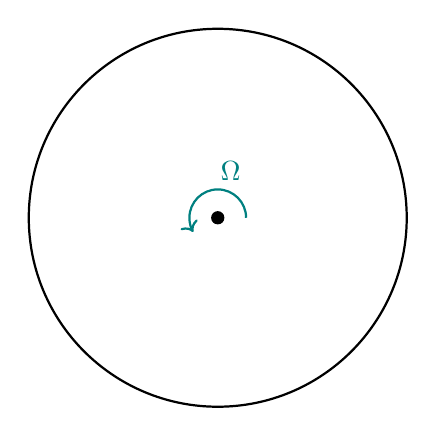
\begin{tikzpicture}[scale=1.2]

    % We want to look above  a rotating table rotating counter clockwise with a pendulum bob orbiting at the axis of rotation at a radius $R$
    % Draw the table
    \draw[thick] (0,0) circle (2); % Table top
    % draw a dot in the center:
    \fill[black] (0,0) circle (2pt); % Center of rotation
    % draw a circular arrow around the center of rotation and label it $\Omega$
    \draw[->, thick, teal] (0.3,0) arc[start angle=0, end angle=210, radius=0.3] node[midway, above right] {$\Omega$};

\end{tikzpicture}

\end{document}
